\label{chapter:conceitos}
Este capítulo tem como objetivo apresentar as principais ferramentas e conceitos que serão utilizadas no desenvolvimento da Hand.io. 


%----------------------------------
% Sistemas Embarcados
%----------------------------------
\section{Sistemas Embarcados}%ok
De acordo com~\citeonline{VAHID:2001} um sistema embarcado é um sistema computacional desenvolvido para um propósito específico, que em contraposição a sistemas de propósito geral, realiza apenas uma tarefa. Existem certas características que distinguem um sistema embarcado dos demais, que apesar de nem sempre serem atendidas, servem de referência para a classificação de tais sistemas. Sistemas embarcados geralmente realizam apenas uma atividade repetidas vezes, contam com restrições mais apertadas que um sistema normal, são reativos e muitas vezes funcionam em tempo real. Estes sistemas geralmente fazem parte de sistemas maiores, e quase sempre funcionam sem o conhecimento do usuário.

Dispositivos como smartphones e computadores pessoais, são compostos por diversos sistemas embarcados que realizam apenas uma função, mas que quando estão juntos passam a realizar diversas atividades, passando a ser classificado como um sistema de propósito geral. Um exemplo de um sistema embarcado que faz parte de um sistema maior seria a placa de rede de um smartphone~\cite{qualcomm_2017}, que por si só é um sistema que apenas recebe e envia dados através de uma rede sem fio, mas que quando contextualizado em um smartphone possibilita o acesso a internet, o que promove a realização de diversas atividades disponíveis online, como acesso à redes sociais ou a reprodução de vídeos.

\todo{adicionar imagem}

\subsection{Restrições de um Sistema Embarcado} %OK

Um sistema embarcado geralmente trabalha em condições restritas nas quais certas métricas devem ser cumpridas para que seu funcionamento se dê de maneira eficiente, em seu livro, \citeonline{marwedel:2011} define uma série de métricas utilizadas para medir a eficiência de um dado sistema como:consumo energético, eficiência em tempo de execução, tamanho de código, peso e custo. Em alguns casos existem situações onde estas métricas entram em conflito, neste caso cabe ao projetista do sistema definir qual a melhor configuração abrindo mão de certas funcionalidades para melhor atender as necessidades da aplicação.

O consumo de energia em um sistema embarcado muitas vezes é limitado devido à tecnologia atual de baterias e ao tipo do circuito utilizado, circuitos integrados desenvolvidos especificamente para certas aplicações tendem a ter uma eficiência energética muito superior aos demais, no entanto abrem mão de flexibilidade no desenvolvimento do software do sistema, circuitos reconfiguráveis como FPGAs\footnote{Field programable gate arrays} tem sua eficiência energética inferior aos ASICs mas oferecem uma flexibilidade de desenvolvimento muito maior apesar são limitados pelo tamanho dos circuitos reconfiguráveis.

A limitação entre flexibilidade e eficiência também se aplica aos processadores. Processadores desenvolvidos especificamente para processamento de sinais analógicos, por exemplo, são exponencialmente mais eficientes energeticamente que processadores de propósito geral, que contam com a pior eficiência energética dentre os circuitos apresentados, mas permitem uma grande gama de possibilidades durante o desenvolvimento do sistema.

As limitações em tempo de execução devem ser reduzidas ao máximo para aproveitar o hardware disponível da melhor maneira possível, problemas acarretados por compiladores que geram binários que não utilizam todo o potencial da arquitetura devem ser corrigidos para afim desperdícios de instruções por ciclo de processamento.

O tamanho do código e as limitações em espaço de armazenamento são um desafio recorrente no mundo dos sistemas embarcados, em diversas aplicações onde não existe a possibilidade de carregamento dinâmico de dados, como ocorrem nos smartphones, todos os dados devem ser armazenados na memória limitada dos chips, como nos casos de Systems on a Chip SoC, nos quais todos os componentes de processamento de dados se encontram em um único chip, nesse tipo de situação onde o espaço se torna um recurso precioso é necessário um cuidado maior durante a construção do código que será executado na plataforma. Tal limitação pode ser contornada com a utilização de memórias flash, mas em certas aplicações devido à outras limitações este tipo de recurso pode não estar disponível.

O peso dos componentes pode ser o fator decisivo na aplicação de um sistema embarcado, existem situações onde o sistema deve ser portátil, logo um peso elevado acabaria por dificultar o manuseio do protótipo, nestes casos o projetista deve ter preferência pelos componentes de tamanho mais reduzido possível.

Em sistemas voltados para o mercado de consumo onde existe um orçamento limitado para o desenvolvimento do sistema, o custo passa a ser uma métrica crucial para o projeto, componentes que não melhoram de maneira significativa a eficiência do pior caso do sistema devem ser descartados afim de reduzir o consumo total de energia. Os requisitos da aplicação devem ser cumpridos utilizando o menor número de componentes possível e com os componentes mais baratos possíveis desde que não comprometam a qualidade do produto final.

\subsection{Sistemas de Tempo Real} %OK

Conforme~\citeonline{BUTTAZZO:2011}, um sistema em tempo real deve ter o tempo do sistema medido utilizando a mesma escala de tempo do mundo real, isto ocorre pelo fato de que o sistema deve ter ciência do ambiente no qual ele irá operar. Sistemas em tempo real geralmente contam com uma definição errônea do seu funcionamento, que diz que um sistema em tempo real deve reagir à estímulos externos com uma certa rapidez e que apenas tendo sido este requisito atendido é o suficiente para que o sistema receba tal classificação, no entanto a definição de tal sistema é mais complexa que apenas esta, o que demonstra que existe um consenso errado sobre o que realmente é um sistema em tempo real.

\citeonline{BUTTAZZO:2011} realiza uma comparação entre sistemas biológicos e a velocidade das suas reações em seus habitats, um gato e uma tartaruga, por exemplo, podem ter velocidades de reação diferentes, no entanto em seus respectivos ambientes esta velocidade se mostra suficiente para a sua sobrevivência. No entanto com mudanças ambientais nas quais não há tempo suficiente para a evolução de suas reações, como a introdução de novos predadores, podem colocar em risco a sobrevivência de organismos já bem estabelecidos em um determinado bioma. Tal exemplo demonstra que o conceito de tempo não é natural aos sistemas, sejam eles biológicos ou artificiais, mas que na verdade está relacionado com o ambiente no qual estes sistemas irão atuar como apresentado na~\autoref{fig:rt}.

\begin{figure}[h]
	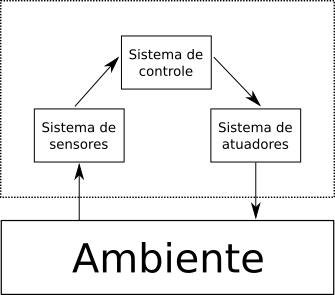
\includegraphics[width=0.5\textwidth, keepaspectratio]{sistemas_em_tempo_real}
    \centering
    \caption{Diagrama de um sistema em tempo real genérico. (Adaptado de~\citeonline{BUTTAZZO:2011})}
    \label{fig:rt}
\end{figure}

Existe um certo consenso na comunidade de que a evolução rápida no processamento de dados irá tornar a utilização de sistemas em tempo real obsoleta, no entanto tal afirmação não poderia estar mais enganada, apesar da computação mais rápida reduza sim o tempo de resposta de um sistema, ela não necessariamente garante que o tempo de resposta de tarefas individuais será atingido de maneira correta, um sistema em tempo real não deve apenas ser rápido, ele deve ser previsível. Analisando os sistemas do ponto de vista de processos, os processos de um sistema em tempo real contam com um componente ausente em processos de sistemas normais, o chamado \textit{Deadline}, que é o prazo máximo para a finalização de uma determinada tarefa. Em aplicações criticas o retorno de operações fora deste deadline não é apenas atrasado, mas sim errado, o que pode ocasionar em perdas significativas dependendo da criticidade do sistema.

A criticidade de uma aplicação depende das consequências ocasionadas devido ao atraso no tempo de resposta esperado do sistema, sendo este classificado em \textit{Hard}, \textit{Firm} e \textit{Soft}.
\begin{itemize}
\item Sistemas críticos \textit{Hard} são aqueles onde caso não haja resposta no tempo definido podem ocorrer eventos devastadores, muitas vezes com perda de vidas.
\item Sistemas críticos \textit{Firm} são aqueles onde o atraso na resposta torna o sistema inútil, no entanto nenhum dano é gerado.
\item Sistemas críticos \textit{Soft} são aqueles onde resultados após o tempo de resposta definido ainda tem alguma utilidade para o sistema, mesmo gerando perda de desempenho.
\end{itemize}

A grande maioria dos sistemas trabalham de maneira hibrida quanto a sua criticidade, onde certas atividades podem ser consideradas como \textit{Hard} e outras podem ser \textit{Soft} ou \textit{Firm}. Atividades com criticidade \textit{Hard} incluem: coleta de dados utilizando sensores, detecção de condições críticas, filtragem de dados, etc. Atividades que contam com com uma criticidade \textit{Firm} podem ser encontradas em aplicações de redes e multimídia, por exemplo: processamento de imagem on-line, execução de vídeos e decodificação de áudio e vídeo. Já atividades com criticidade \textit{Soft} geralmente estão relacionadas à interação com o usuário como: a exibição de mensagens em uma tela, o processamento de sinais de teclado e o armazenamento de dados de utilização.

A luva Hand.io é um sistema de tempo real que trabalha com atividades com criticidade \textit{Firm}, pois a falha no reconhecimento de um gesto e a realização da ação correspondente a este, não gera perdas de vidas ou perdas financeiras significativos, apenas tornam o sistema inútil.


%----------------------------------
% MICROS
%----------------------------------
\subsection{Microcontroladores e Microprocessadores}%ok

As diferenças entre microcontroladores e microprocessadores são apresentadas por \citeonline{ayala:1991} em seu livro, onde fica claro que apesar de terem surgido da mesma ideia e serem fabricados pelo mesmo grupo de pessoas, seu funcionamento e aplicação diferem grandemente. Existem diferenças fundamentais no design de tais dispositivos, enquanto microcontroladores por si só contam com todos os componentes necessários para o seu funcionamento, microprocessadores necessitam de outros componentes e periféricos para funcionar como um computador completo.

Microprocessadores são conhecidos popularmente como Unidades Centrais de Processamento (CPU, em inglês), e tem como sua função principal buscar e modificar extensivamente dados da memória para que sejam armazenados ou exibidos para o usuário. Por si só um microprocessador não constitui um microcomputador completo, para se tornar uma máquina capaz de executar programas de propósito geral se faz necessária a utilização de memórias RAM, memórias de armazenamento massivo e diversos dispositivos de entrada e saída externos. O termo que melhor descreve microprocessadores seria \textit{propósito geral}, o hardware destes componentes é desenvolvido de tal maneira a permitir o desenvolvimento de sistemas grandes ou pequenos dependendo da demanda da aplicação. O design do microprocessador é desenvolvido a fim de cumprir as suas expectativas no mercado de consumo em massa.

Os microcontroladores funcionam de maneira similar aos microprocessadores, no entanto além de terem os componentes encontrados em um microprocessador eles também contam com todos os componentes necessários para o funcionamento de um computador completo, como memórias RAM, memórias ROM e portas paralelas e seriais de entrada e saída. Como os microprocessadores, os microcontroladores também são componentes de propósito geral, mas o seu foco deixa de ser apenas computar os dados encontrados na memória e armazena-los, e passa também controlar o ambiente em que se encontram se baseando nos resultados do processamento dos dados disponíveis. Os programas utilizados em microcontroladores são armazenados na memória ROM e não tem seu funcionamento alterado durante o ciclo de vida do sistema. As instruções de máquina encontradas nos microcontroladores geralmente envolvem buscar dados na memória interna e que também realizam operações envolvendo os pinos inclusos na plataforma, o que permite que cada pino tenha seu propósito programado de acordo com a vontade do desenvolvedor.


%----------------------------------
% VSS
%----------------------------------

\section{Modelagem de sistemas}

\subsection{UML}

\section{Verificação de Software e Hardware}

Segundo \citeonline{edwards:1997} 

\subsection{Modelos Formais}



\subsection{Máquina de Estados}


\subsection{Rede de Petri}
~\citeonline{VALK:2002}



%----------------------------------
% IoT
%----------------------------------
\section{Internet das Coisas}

No trabalho de~\citeonline{ATZORI:2010} é demonstrado que em sua ideia fundamental a internet das coisas é um ambiente de computadores pervasivos que interagem um com os outros de maneira cooperativa para atingir metas em comum, este conceito permite a idealização de ambientes inteligentes onde todos os objetos estão em constante comunicação: para auxiliar o usuário a atingir uma qualidade de vida maior.

Nos ambientes residenciais e empresariais, a internet das coisas pode tornar a vida muito mais confortável e eficiente com sensores e atuadores, coletando dados sobre a preferência dos usuários e sobre o clima é possível que a temperatura seja adequada automaticamente levando em consideração o gasto de energia elétrica para uma maior economia.

%----------------------------------
% IA
%----------------------------------
\section{Reconhecimento de Padrões}



\subsection{Aprendizagem de Máquina}

Segundo \citeonline{norvig:780391} o aprendizado ocorre quando um agente, seja ele uma máquina ou um humano, melhora sua performance em tarefas futuras após realizar observações do ambiente no qual ele atua se baseando em pares de entradas e saídas para prever novas saídas a partir de novas entradas.

A utilização do aprendizado de máquina se justifica pela necessidade de criar sistemas adaptativos, pois durante o desenvolvimento muitas vezes não é possível prever mudanças que podem ocorrer no ambiente no qual o sistema irá atuar, ou mesmo porquê não é possível de maneira simples se desenvolver um sistema que possa atender as necessidades da aplicação utilizando métodos tradicionais de programação.

De acordo com \citeonline{norvig:780391} existem três tipos de aprendizado que diferem no tipo de \textit{feedback} informado ao agente que busca se aprimorar. No aprendizado não-supervisionado o agente busca aprender padrões nas entradas de dados sem que qualquer tipo de \textit{feedback} seja informado de maneira explícita. O tipo mais comum de atividade deste tipo de aprendizado seria a criação de grupos a partir de entradas, por exemplo, um cachorro pode desenvolver uma noção sobre dias de passear ou dias de ficar em casa de acordo com o clima do dia sem que o seu dono tenha explicitamente dito que era a hora de passear.

No aprendizado por reforço o agente aprende a partir de incentivos ou punições que são aplicados de acordo com o resultado da predição de saídas a partir de novas entradas. Um exemplo deste tipo de aprendizado seria quando o dono de um cachorro tenta ensinar novos truques a ele oferecendo um biscoito quando ele realiza o truque de maneira correta, e falando com uma voz mais firme sem oferecer o biscoito quando ele realiza o truque de maneira incorreta.

No aprendizado supervisionado o agente observa pares de entradas e saídas e tenta criar novas funções para reproduzir estes resultados a partir de novas entradas. Um exemplo deste tipo de aprendizado acontece quando uma criança é ensinada sobre como realizar cálculos matemáticos simples e o professor apresenta exemplos de cálculos corretos esperando que a criança realize o mesmo cálculo com valores diferentes e resultados diferentes por si só, sendo informada se o resultado estava correto ou não.

\subsubsection{SciKitLearn}

\subsubsection{TensoFlow}
